% !TEX TS-program = pdflatex
% !TEX encoding = UTF-8 Unicode

% This is a simple template for a LaTeX document using the "article" class.
% See "book", "report", "letter" for other types of document.

\documentclass[18pt]{article} % use larger type; default would be 10pt

\usepackage[utf8]{inputenc} % set input encoding (not needed with XeLaTeX)

%%% Examples of Article customizations
% These packages are optional, depending whether you want the features they provide.
% See the LaTeX Companion or other references for full information.

%%% PAGE DIMENSIONS
\usepackage{geometry} % to change the page dimensions
\geometry{a4paper} % or letterpaper (US) or a5paper or....
% \geometry{margin=2in} % for example, change the margins to 2 inches all round
% \geometry{landscape} % set up the page for landscape
%   read geometry.pdf for detailed page layout information
\setlength{\parindent}{0pt}


% \usepackage[parfill]{parskip} % Activate to begin paragraphs with an empty line rather than an indent

%%% PACKAGES
\usepackage{booktabs} % for much better looking tables
\usepackage{array} % for better arrays (eg matrices) in maths
\usepackage{paralist} % very flexible & customisable lists (eg. enumerate/itemize, etc.)
\usepackage{verbatim} % adds environment for commenting out blocks of text & for better verbatim
\usepackage{subfig} % make it possible to include more than one captioned figure/table in a single float
\usepackage{amsmath} %amsmath is part of AMS-LATEX bundles
\usepackage{amssymb}%symble
\usepackage{amsfonts}%font
\usepackage{amsthm}%provide theorem package
\usepackage{graphicx}
\usepackage{listings}
% These packages are all incorporated in the memoir class to one degree or another...
\usepackage[retainorgcmds]{IEEEtrantools} %In order to use IEEEeqnarray Environment
\usepackage{graphicx} % support the \includegraphics command and options
%\usepackage{indentfirst}%

%%% HEADERS & FOOTERS
\usepackage{fancyhdr} % This should be set AFTER setting up the page geometry
\pagestyle{fancy} % options: empty , plain , fancy
\renewcommand{\headrulewidth}{0pt} % customise the layout...
\lhead{}\chead{}\rhead{}
\lfoot{}\cfoot{\thepage}\rfoot{}

%%% SECTION TITLE APPEARANCE
\usepackage{sectsty}
\allsectionsfont{\sffamily\mdseries\upshape} % (See the fntguide.pdf for font help)
% (This matches ConTeXt defaults)

%%% ToC (table of contents) APPEARANCE
\usepackage[nottoc,notlof,notlot]{tocbibind} % Put the bibliography in the ToC
\usepackage[titles,subfigure]{tocloft} % Alter the style of the Table of Contents
\renewcommand{\cftsecfont}{\rmfamily\mdseries\upshape}
\renewcommand{\cftsecpagefont}{\rmfamily\mdseries\upshape} % No bold!

%%%DEFINE UPRIGHT FONT MISSING FUNCTIONS????????????????????
\DeclareMathOperator{\argh}{argh}
\DeclareMathOperator*{\nut}{Nut}

%%%DEFINE NEW COMMANDS
\newcommand{\ud}{\,\mathrm{d}}

%%%DEFINE THEOREM
%\theoremstyle{definition} 
\theoremstyle{definition}\newtheorem{law}{Law}
\theoremstyle{plain}\newtheorem{jury}[law]{Jury}
\theoremstyle{remark}\newtheorem{juu}{Juu}
\theoremstyle{definition}\newtheorem{kuu}[law]{Kuu}
\theoremstyle{definition}\newtheorem{muu}{Muu}[section]
\theoremstyle{definition}\newtheorem{honoluu}{Honoluu}[section]
\theoremstyle{definition}\newtheorem{konoluu}[muu]{Konoluu}

%%% END Article customizations

%%% The "real" document content comes below...

\title{\textbf{ \begin{LARGE}CSE150:Introduction to Artificial Intelligence\end{LARGE}}\\ [0ex]\begin{Large} Homework 4 \end{Large} }
\author{Ning Ma}
\date{} % Activate to display a given date or no date (if empty),
         % otherwise the current date is printed 

\begin{document}

\begin{figure}[htbp]
\centering
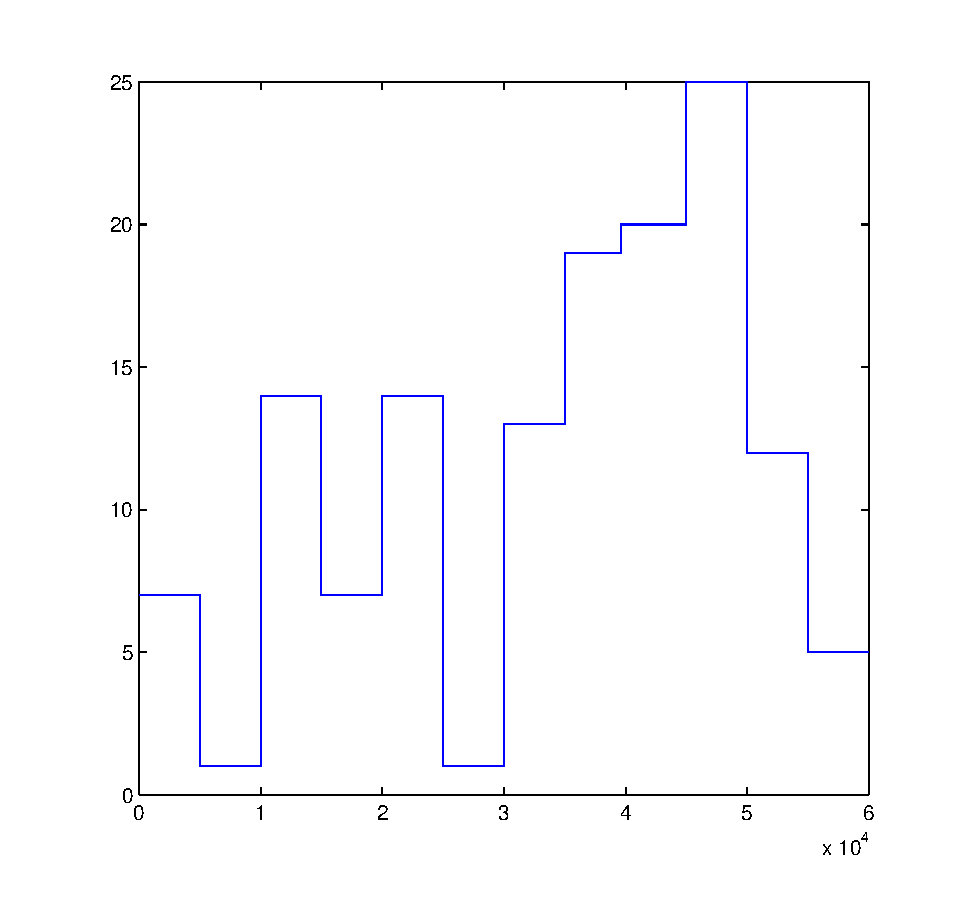
\includegraphics[width=0.8\textwidth]{S_STAR.eps}
\caption{Most likely sequence}
\label{LLH1}
\end{figure}
The sequence is \textbf{gangnamstyle}

The following is the Matlab source code\\

\begin{lstlisting}
//
//  main.cpp
//  cs_hw5_verbiti
//
//  Created by Ning Ma on 2/23/13.
//  Copyright (c) 2013 Ning Ma. All rights reserved.
//
#include <iomanip>
#include <iostream>
#include <fstream>
#include <sstream>// for istringstream
#include <vector>
#include <set>
#include <algorithm>
#include <cmath>

using namespace std;

//read initial data from the txt files
void initialize(string a, vector<vector<double> >& matrix) 
{
    string line;    vector<double> row;
    double number = 0;
    ifstream myfile;
    myfile.open(a);
    if(!myfile)
    {
        cout << "can't open or find the file" << endl;
        exit(1);
    }
    while(getline(myfile,line))//get next line from the file
    {
        
        if(line.empty())
            continue;
        istringstream inputstream(line);//separtae the line based on the spaces between words
        row.clear();
        
        while( inputstream >> number )
        {
            //cout << number << " ";
            row.push_back(number);//get a row of matrix
        }
        //cout << endl;
        matrix.push_back(row);//get the matrix
    }
    myfile.close();
    
}


int main(int argc, const char * argv[]) 
{

    //L_matrix : compute the matrix L_it;
    //Theta_matrix : the matrix which record the most likely transition
    vector<vector<double> >  Ini_state, A_transition, B_emission, O_observation;
    vector<double> temp_column;
    vector<vector<double> >::iterator iter_r;
    vector<double>::iterator iter;
    double max_value;
    
    typedef const vector<double>::size_type CONST_vec_sz;
    typedef const vector<vector<double> >::size_type CONST_vec_vec_sz;
    typedef vector<double>::size_type vec_sz;
    typedef vector<vector<double> >::size_type vec_vec_sz;
    vec_vec_sz j, i;
    vec_sz t, max_index;
    
    initialize("emissionMatrix.txt", B_emission);
    initialize("initialStateDistribution.txt", Ini_state);
    initialize("transitionMatrix.txt", A_transition);
    initialize("observations.txt",O_observation);
    
    CONST_vec_vec_sz N_state = Ini_state.size();//number of states
    CONST_vec_sz T = O_observation[0].size(); //number of obervations
    cout << N_state << " " << T << endl;
    vector<vector<double> >L_matrix(N_state, vector<double>(T));
    vector<vec_sz> S_star(T);
    vector<vector<vec_sz> > Theta_matrix(N_state, vector<vec_sz>(T));
    
    temp_column.clear();
    for(i = 0; i < N_state; i++)
    {
        L_matrix[i][0] = log( Ini_state[i][0] ) + log( B_emission[i][O_observation[0][0]] );
        //cout << L_matrix[i][0] << endl;
    }
    for( t = 1; t < T; t++ )
    {
        for ( j = 0; j < N_state; j++)
        {
            
            for( i = 0; i < N_state; i++)
            {
                temp_column.push_back(L_matrix[i][t-1] + log(A_transition[i][j]));
                //cout << temp_column[i] <<endl;
            }
            
            iter = max_element( temp_column.begin(),temp_column.end() );
            max_index = iter - temp_column.begin();
            max_value = *iter;
            L_matrix[j][t] = max_value + log(B_emission[j][O_observation[0][t]]);
            Theta_matrix[j][t] = max_index;
            temp_column.clear();
            //cout << Theta_matrix[j][t] << endl;

        }
        

    }
    //cout << Theta_matrix[16][2] << endl;
    for(i = 0; i < N_state; i++)
        temp_column.push_back(L_matrix[i][T-1]);
    iter = max_element( temp_column.begin(),temp_column.end() );
    max_index = iter - temp_column.begin();
    S_star[T-1] = max_index+1;
    cout << S_star[T-1] << endl;
    
    for (t = T-2; t > 0; t--)
    {
        S_star[t] = Theta_matrix[S_star[t+1]-1][t+1]+1;
        //cout << S_star[t] << " " << t << endl;
    }
    S_star[0] = Theta_matrix[S_star[1]][1];
    /*for(i = 0; i < O_observation.size(); i++)
    {
        row = O_observation[i];
        for (j = 0; j < row.size(); j++)
        {
            cout << row[j] << " ";
        }
        cout << endl;
        
    }*/
    ofstream outfile;
    outfile.open("S_star.txt");
    if(!outfile)
        cout << "can't open a file" <<endl;
    for (t = 0;t < T;t++)
        outfile << S_star[t] <<endl;
    outfile.close();

    return 0;
}
\end{lstlisting}
\end{document}
